\section{Аналитическая часть}
\subsection{Основные понятия}
\textbf{Потоковый трафик} -- тип трафика, для которого характерен просмотр и/или прослушивание информации по мере её поступления на конечное оборудование (мобильный телефон, компьютер, телевизор с доступом в Интернет и т.д.). \cite{stream_traffic} Основную часть потокового трафика составляет потоковое видео (или видеопоток).

\textbf{Видеостриминг} (или \textbf{стриминг видео}) -- технология передачи видеоконтента через Интернет в режиме реального времени, при этом пользователь не должен ждать полной загрузки файла для просмотра. \cite{video_streaming} Видео транслируется непрерывным потоком в виде последовательных кадров в специальном формате. Просмотр начинается в момент достаточной буферизации, обеспечивая при этом равномерное отображение данных. 

Основой для передачи мультимедийной информации в настоящее время становятся мультисерверные платформы. Они способны отправлять данные разных типов и поддерживать трафик с различными характеристиками. Наибольшее распространение получили два варианта передачи потокового видео по сети.
\begin{itemize}
	\item \textit{Видео реального времени (real-time streaming)}, запись которого осуществляется одновременно с его просмотром, например, видеоконференции, прямые эфиры.
	
	\item \textit{Видео по запросу} (progressive streaming). Предварительно записанные видеоряды хранятся на сервере, запрашиваются приложениями конечного пользователя и воспроизводятся при получении.
\end{itemize}

Привлечение мультипоточной загрузки, при которой данные загружаются сразу с нескольких серверов или источников, имеет следующие преимущества по сравнению с загрузкой только с одного сервера.
\begin{itemize}
	\item \textit{Увеличение скорости загрузки}. Мультипоточная загрузка позволяет использовать полную пропускную способность нескольких серверов одновременно, ускоряя процесс передачи видеоконтента. Это особенно полезно при работе с большими файлами, например, с видео высокого разрешения.
	
	\item \textit{Улучшение стабильности и отказоустойчивости}. Если один из источников недоступен или работает медленно по какой-то причине, то другие могут продолжать предоставлять необходимые данные. Это минимизирует возможные проблемы с недоступностью серверов.
	
	\item \textit{Оптимизация использования сетевых ресурсов}. Разделение загрузки данных между несколькими серверами помогает избежать перегрузки одного сервера и эффективно использовать сетевые ресурсы.
	
	\item \textit{Адаптация к сетевым ограничениям}. При привлечении нескольких серверов можно адаптировать процесс загрузки к изменениям сетевых условий (например, изменение скорости интернет-соединения), что помогает поддерживать стабильное и качественное воспроизведение. 
\end{itemize}

Все эти преимущества делают мультисерверную загрузку более предпочтительной, особенно в случаях, если важна скорость передачи данных, стабильности и отказоустойчивость системы.

Как правило, система трансляции потоковых видео состоит из четырёх подсистем:
\begin{enumerate}
	\item \textbf{Устройство кодирования} для сжатия видеопотока и загрузки его на медиасервер. 
	
	\item \textbf{Медиасервер}, отвечающий за хранение видеорядов и передачу пользователям. Он является ключевой единицей во всём процессе передачи. Основная его задача -- взаимодействие с транспортной сетью при отправке пакетов в нужное время. Как правило, состоит из трёх компонентов механизма трансляции: \textit{транспортный протокол, операционная система и система хранения}.
	
	\item \textbf{Транспортная сеть}, которая транслирует пакеты от медиасервера до клиентского устройства с помощью специально разработанных и стандартизированных протоколов. Последние обеспечивают такие услуги связи, как сетевая адресация, транспортировка и контроль за сеансом связи.
	
	\item \textbf{Клиентское приложение}, декодирующее и воспроизводящее мультимедиапоток. Также опционально может присутствовать механизм синхронизации аудио и видео.
\end{enumerate}

Действующий протокол между клиентом и сервером определяет:
\begin{enumerate}
	\item синтаксис и формат данных \\
	Фиксируется чёткая структура сообщений или пакетов данных, которые передаются между устройствами. Как правило, это описание формата заголовков и тела сообщения.
	
	\item способ установления соединения \\
	Протокол может определять процедуру процессов установления, поддержания и завершения соединения между устройствами. 
	
	\item основные операции и команды \\
	Описывается множество доступных операций, команд или запросов, которые могут быть выполнены в рамках существующего протокола. 
	
	\item обработку ошибок и контроль целостности данных \\
	Определяются методы и сценарии обработки некорректных ситуаций, способы контроля целостности данных.
	
	\item управление потоком данных \\
	Может также описываться алгоритм регулирования скорости передачи потока информации.
\end{enumerate}

В текущей работе будет рассматриваться протокол мультисерверного видеостриминга для передачи данных по запросу. \\

\subsection{Возможные сферы применения и целевая аудитория}
Подобный протокол может быть применён в рамках высоконагруженных систем, позволяя увеличивать скорость загрузки данных путём одновременного запроса и получения разных частей контента с нескольких серверов. Такой подход позволяет не только ускорить загрузку видео, но и обеспечивает более плавное воспроизведение, поскольку некоторые части запрашиваются заранее и в случае потери, могут быть получены повторно. 

Его привлечение в сервисах видеохостинга особенно полезно в случае нестабильного Интернет-соединения и большого объёма файла. Например, разрабатываемый протокол может быть привлечён в рамках обязательного внеурочного занятия в России, введённого в программы образовательных организаций начального, основного, среднего и профессионального образования. Каждый понедельник на первом уроке учащимся показывают видеофайлы, повествующие о наиболее актуальных событиях в стране, на основе которых строится дальнейшее обсуждение поднятых в них тем. 

Таким образом, каждое утро понедельника классные руководители по всей стране скачивают подготовленные ролики с сайта <<Разговоры о важном>>, создавая колоссальную нагрузку на серверы, из-за чего постоянно возникают сбои и сложности с загрузкой. Рассматриваемый в рамках текущей курсовой работы протокол может помочь решить некоторые возникающие проблемы, путём распределения процесса загрузки видеофрагментов по нескольким серверам.

Также его можно привлечь в процессе обмена видеофайлами между платформами для ускорения процесса переноса данных. Это может быть актуально для сервисов, размещающих видео сразу на нескольких платформах, например, YouTube, Rubube, VK Видео. \\

\subsection{Форматы видеорядов}
Наиболее часто встречающиеся форматы видео:
\begin{itemize}
	\item \textbf{MP4 (по-другому MPEG-4 Part 14)} – формат, совместимый с большинством браузеров и поддерживаемый сайтами потокового видео, в частности, YouTube.
	
	\item \textbf{AVI (Audio Video Interleave)} – старый формат, разработанный Microsoft. Поддерживается большинством популярных браузеров, работающих в системах Windows, Linux. 
	
	\item \textbf{MPG, MPEG, MP2, MPE, MPV} – форматы, в которых обычно записывают видео, которые впоследствии не нужно будет редактировать.
	
	\item \textbf{MOV} – формат, разработанный Apple. Видео сохраняется в хорошем качестве, но файл занимает много места.
	
	\item \textbf{WebM} – формат, позволяющий получать видео небольшого размера среднего качества. Видео в таком формате подходят для YouTube и других сайтов потокового видео на платформе HTML5.
\end{itemize}

Формат видео существенно не влияет на протокол видео-трансляции, поэтому в демонстративных целях будет использоваться только MP4, другие видео-форматы также могут быть привлечены при доработках реализации парсера и проигрывателя медиафайла. \\

\subsection{Основные этапы протокола мультисерверного стриминга с множественными источниками}
На рисунке \ref{image:general_process} схематично представлен общий алгоритм работы протокола. Ключевые моменты отмечены цифрами.

\begin{figure}[h]
	\begin{center}
		{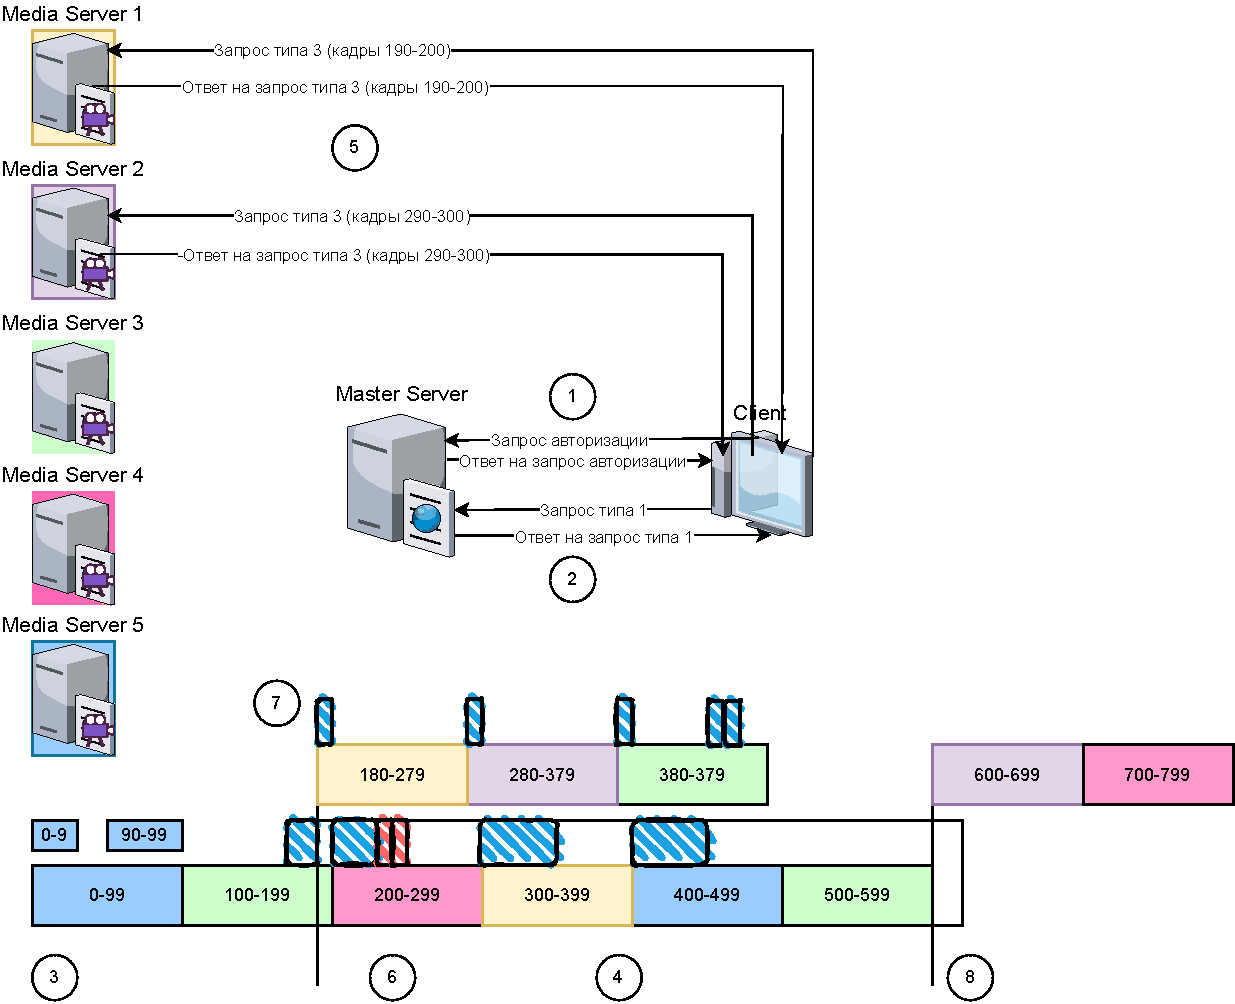
\includegraphics[scale = 0.8]{img/[all process].pdf}}
		\caption{Основные этапы протокола.}
		\label{image:general_process}
	\end{center}
\end{figure}

\pagebreak

Весь видеофайл разбивается на несколько фрагментов (на рисунке метка 3), каждый из которых может быть получен от любого медиа-сервера.

Сначала клиент должен пройти процесс авторизации, обозначен цифрой 1, после успешного завершения он может запросить у мастер-сервера распределение интервалов видео по хостам (отмечен 2). 

Получив его, клиент делает несколько параллельных запросов к различным медиа-серверам (отмечено как 5) на загрузку $n$ кадров.

В случае $m$ неуспешных запросов к какому-либо медиа-серверу (отмечено 6) клиент должен сообщить мастер-серверу о проблеме, инициировав перераспределение фрагментов между хостами. 

Таким образом, клиент получает новый список медиа-серверов с перераспределёнными видео-интервалами загружаемого файла (отмечено на рисунке цифрой 7) и начинает выгрузку ещё не полученных кадров. 

Клиент загружает такой объём информации, который помещается в буфер (отмечен на рисунке цифрой 4). 

Как только окно загрузки будет передвинуто на некоторую величину кадров, клиент должен отправить запрос на получение списка медиа-серверов для новых видео-фрагментов (цифра 8). \\

\subsection*{Выводы}
Таким образом, в данной работе будет разрабатываться протокол для мультисерверного видеостриминга с множественными источниками. В качестве формата видео был выбран MP4. В разделе был описан принцип работы протокола, выделены необходимые виды сообщений. 

















